\documentclass{article}

\usepackage{fancyhdr}
\usepackage{extramarks}
\usepackage{amsmath}
\usepackage{minted}
\usepackage{amsthm}
\usepackage{amsfonts}
\usepackage{tikz}
\usepackage[plain]{algorithm}
\usepackage{algpseudocode}

\usetikzlibrary{automata,positioning}
\usepackage{fullpage,enumitem,amsmath,amssymb,graphicx}

%
% Basic Document Settings
%

\topmargin=-0.75in
\textwidth=6.5in
\textheight=9.0in
\headsep=0.20in
\headheight = 12pt
\linespread{1.1}

\pagestyle{fancy}
\chead{\hmwkClass\ (\hmwkClassInstructor): \hmwkTitle}
\rhead{\firstxmark}
\lfoot{\lastxmark}
\cfoot{\thepage}

\renewcommand\headrulewidth{0.55pt}
\renewcommand\footrulewidth{0.55pt}

\setlength\parindent{0pt}


\setcounter{secnumdepth}{0}

%
% Homework Problem Environment
%
% This environment takes an optional argument. When given, it will adjust the
% problem counter. This is useful for when the problems given for your
% assignment aren't sequential. See the last 3 problems of this template for an
% example.

%
% Homework Details
%   - Title
%   - Due date
%   - Class
%   - Section/Time
%   - Instructor
%   - Author
%

\newcommand{\hmwkTitle}{Homework\ \#4}
\newcommand{\hmwkDueDate}{October 01, 2021}
\newcommand{\hmwkClassCode}{COT 5615}
\newcommand{\hmwkClass}{Math for Intelligent Systems}
\newcommand{\hmwkClassYear}{Fall 2021}
\newcommand{\hmwkClassInstructor}{Professor Kejun Huang}
\newcommand{\hmwkAuthorName}{\textit{Vyom Pathak}}
\newcommand{\hmwkUFID}{96703101}

%
%
%
% Various Helper Commands
%

% Useful for algorithms
\newcommand{\alg}[1]{\textsc{\bfseries \footnotesize #1}}

% For derivatives
\newcommand{\deriv}[1]{\frac{\mathrm{d}}{\mathrm{d}x} (#1)}

% For partial derivatives
\newcommand{\pderiv}[2]{\frac{\partial}{\partial #1} (#2)}

% Integral dx
\newcommand{\dx}{\mathrm{d}x}

% Alias for the Solution section header
\newcommand{\solution}{\textbf{\large Solution}}

% Probability commands: Expectation, Variance, Covariance, Bias
\newcommand{\E}{\mathrm{E}}
\newcommand{\Var}{\mathrm{Var}}
\newcommand{\Cov}{\mathrm{Cov}}
\newcommand{\Bias}{\mathrm{Bias}}

% norm bars
\newcommand{\norm}[1]{\left\lVert#1\right\rVert}

\begin{document}

\begin{center}
{\Large \hmwkClassCode\ \hmwkClass\ \hmwkClassYear\ \hmwkTitle}

\begin{tabular}{rl}
UFID: & \hmwkUFID \\
Name: & \hmwkAuthorName \\
Instructor: & \hmwkClassInstructor \\
Due Date: & \hmwkDueDate \\ 
% Collaborators: & [list all the people you worked with]
\end{tabular}
\end{center}

\section*{Problem 7.6}
\subsection*{Rows of incidence matrix}
\subsubsection*{Solution}
According to the definition of incidence matrix, the sum of the rows will be equal to zero, $1^TA=0$, and thus the rows of the incidence matrix are always linearly dependent.
\section*{Problem 7.8}
\subsection*{Flow conservation with sources}
\subsubsection*{Solution}
Here, we can prove $1^Ts=0$ by the following derivation:
\begin{align*}
    Ax+s & = 0\\
    1^T(Ax+s) & = 1^T0\\
    (1^TA)x + 1^Ts & = 0\\
    0+1^Ts & = 0\ \ (\because 1^TA=0)\\
    \therefore 1^Ts & =0
\end{align*}
\section*{Problem 7.15}
\subsection*{Channel equalization}
\subsubsection*{Solution}
\begin{enumerate}[label=\alph*]
    \item Here, using the associative property of convolution we get the following result:
    \begin{align*}
        z & = h*y\\
        z & = h*(c*u)\\
        z & = (h*c)*u\\
        z & \approx e_1*u\ \ (\because given)\\
        z & \approx (u_1,u_2,\ldots,u_m,0,0,\ldots,0)
    \end{align*}
    \item Following is the code for calculation and plotting u, y, z with sizes 50, 52, and 59 respectively.
    \begin{minted}[
frame=lines,
framesep=2mm,
baselinestretch=1.2,
fontsize=\footnotesize,
linenos
]{julia}
    using LinearAlgebra
    using DSP
    using Random
    using Plots
    plotly()
    rng = MersenneTwister(1234);
    u = shuffle(rng, Vector(1:50))
    X = -1;
    Y = +1;
    C = findall(u.<=25);
    D = findall(u.>25);
    u[C] .= X;
    u[D] .= Y;
    c = [1,0.7,-0.3];
    h = [0.9, -0.5, 0.5, -0.4, 0.3, -0.3, 0.2, -0.1];
    y = conv(c,u);
    z = conv(h,y);
    plot(1:length(u),u)
    plot(1:length(y),y)
    plot(1:length(z),z)
    \end{minted}
Following are the generated graphs:
\begin{figure}[htp]
\centering
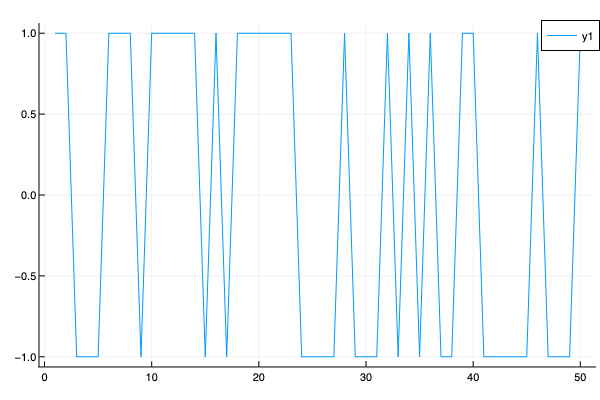
\includegraphics[width=.3\textwidth]{u.png}\hfill
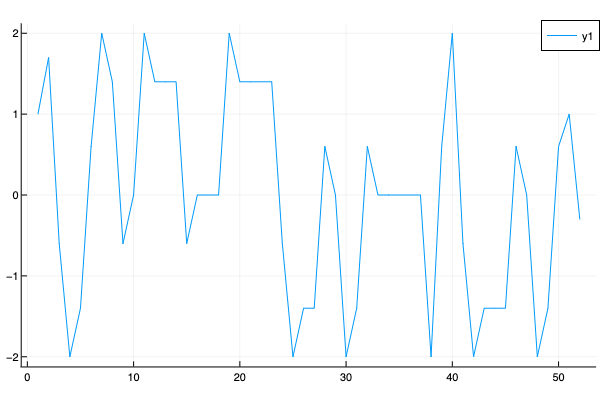
\includegraphics[width=.3\textwidth]{y.png}\hfill
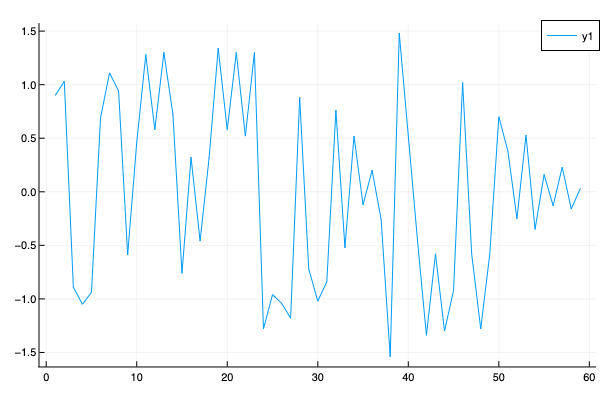
\includegraphics[width=.3\textwidth]{z.png}
\caption{signal v/s t for u, y and z respectively.}
\label{fig:figure3}
\end{figure}
\end{enumerate}
\section*{Problem A7.1}
\subsection*{Equalization in communication}
\subsubsection*{Solution}
\begin{minted}[
    frame=lines,
    framesep=2mm,
    baselinestretch=1.2,
    fontsize=\footnotesize,
    linenos
    ]{julia}
    include("channel_equalization_data.jl")    
    hc = conv(h,c);
    y = conv(c,s);
    y_tilda = conv(h,y);
    
    plot(1:length(c), c)
    plot(1:length(h), h)
    plot(1:length(hc), hc)
    
    plot(1:length(s[1:100]), s[1:100])
    plot(1:length(y[1:100]), y[1:100])
    plot(1:length(y_tilda[1:100]), y_tilda[1:100])
    
    s_cap = 1*(y .> 0.5);
    s_cap_eq = 1*(y_tilda .> 0.5);
    BER = sum( broadcast(abs, s_cap[1:1000]-s))/1000;
    BER_eq = sum( broadcast(abs, s_cap_eq[1:1000]-s))/1000;
    println("Bit Error rate for non-equilized transmission signal: ",BER) #0.113
    println("Bit Error rate for equilized transmission signal: ",BER_eq) #0.0
    \end{minted}

\begin{figure}[htp]
\centering
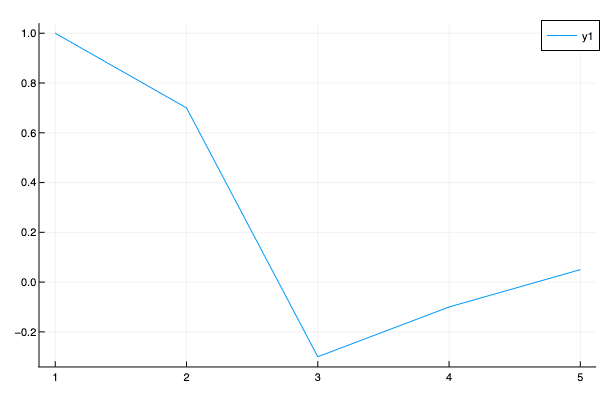
\includegraphics[width=.3\textwidth]{c_7.1.png}\hfill
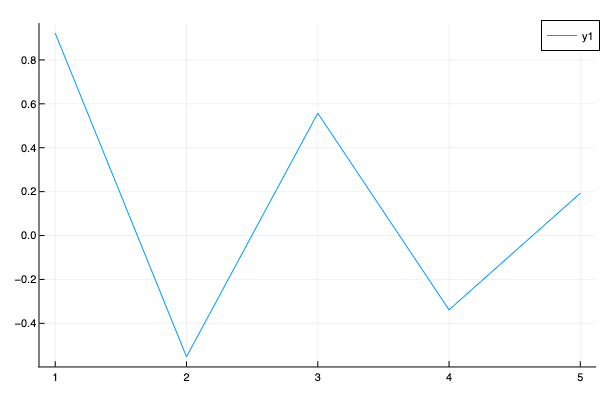
\includegraphics[width=.3\textwidth]{h_7.1.png}\hfill
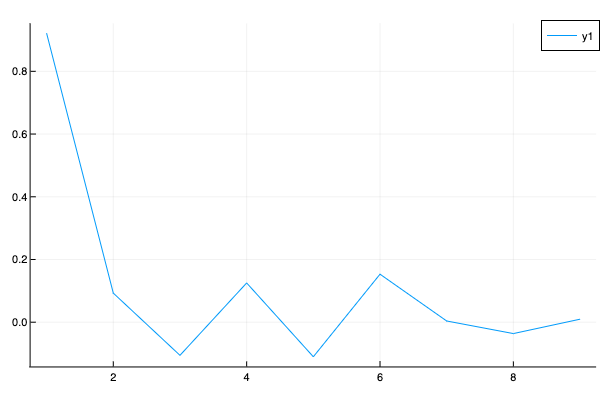
\includegraphics[width=.3\textwidth]{hc_7.1.png}
\caption{signal v/s t for c, h and h*c respectively.}
\label{fig:figure4}
\end{figure}
\begin{figure}[htp]
\centering
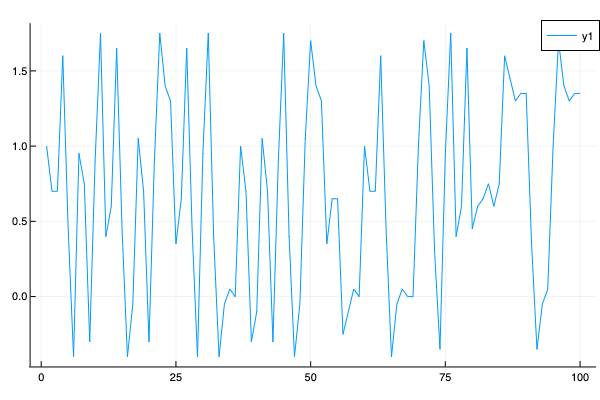
\includegraphics[width=.47\textwidth]{y_7.1.png}\hfill
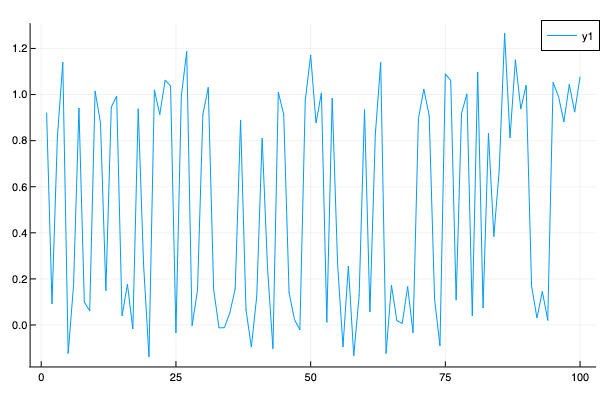
\includegraphics[width=.47\textwidth]{y_tilda_7.1.png}\hfill
\caption{signal v/s t for y and y\_tilda respectively.}
\label{fig:figure5}
\end{figure}
\begin{enumerate}[label=\alph*]
    \item From figure \ref{fig:figure4} we can see that channel impulse response $c$ has some amount of noise. After equalization of the channel impulse response $h*c$, we can see that sufficient amount of noise is reduced while minimizing the effects of the interference.
    \item From figure \ref{fig:figure5}, it is a little bit clear that \^{s} will be a worse estimate of s than \^{s}$^{eq}$.
    \item The BER for \^{s}=0.113 and BER for \^{s}$^{eq}=0.0$, which proves that equalized signal is better than non-equalized signal for estimating the transmitted message.
\end{enumerate}
\section*{Problem A7.3}
\subsection*{Audio Filtering}
\subsubsection*{Solution}
    \begin{minted}[
frame=lines,
framesep=2mm,
baselinestretch=1.2,
fontsize=\footnotesize,
linenos
]{julia}
    using WAV
    x, f = wavread("audio_filtering_original.wav");
    x = vec(x);
    #a) 
    h_smooth = 1 / 44 * ones(44);
    output = conv(h_smooth, x);
    wavplay(output, f); #Play Audio
    #b)
    IR = zeros(convert(Int32,round(0.03125*f,digits=0))); #Impulse Response
    IR[1,1] = 1;
    d = f*0.25
    k = 0.5
    drypath = vcat(IR,zeros(convert(Int32,d)));
    wetpath = vcat(zeros(convert(Int32,d)),IR);
    out = zeros(size(drypath));
    for n in 1:length(drypath)
        out[n,1] = drypath[n,1]+k*wetpath[n,1];
    end
    #Here out is the h_echo filter
    echo_IR = conv(out,x); #h_echo*x
    wavplay(echo_IR, f); #Play Audio
    echo_IR_2 = conv(out,echo_IR); #h_echo*h_echo*x
    wavplay(echo_IR_2, f); #Play Audio
\end{minted}
\begin{enumerate}[label=\alph*]
    \item After applying the smooth filter using convolution, the volume of the audio has decreased as well as the sharpness of the audio decreases.
    \item The $h_{echo}$ is an impulse response filter developed to generate an impulse at a given delayed position of given attenuation value. The code for the same can be found above. After applying the echo filter again, more delayed audio with same amplitude is superimposed on the audio and we can hear the echo more clearly.
\end{enumerate}
\section*{Problem 8.7}
\subsection*{Interpolation of polynomial values and derivatives}
\subsubsection*{Solution}
The four equations can be written as follows:
\begin{align*}
    c_1 & = 0\\
    c_2 & = 0\\
    c_1+c_2+c_3+c_4+c_5 & = 1\\
    c_2+2c_3+3c_4+4c_5 & = 0
\end{align*}
These equations can be written as $Ac = b$ as follows:
\begin{align*}
    A = (1,0,1,0; 0,1,1,1; 0,0,1,2; 0,0,1,3; 0,0,1,4), b = (0,0,1,0)
\end{align*}
The set of equations are undetermined as there are only 4 equations and 5 unknown variables.
\section*{Problem 8.11}
\subsection*{Location from range measurements}
\subsubsection*{Solution}
By squaring and expanding on the RHS we get the following:
\begin{align*}
x^Tx-2a_i^T+a_i^Ta_i = \rho_i^2,\ i = 1,2,3,4
\end{align*}
Now subtracting equation 1 from each of the other equations, the term $x^Tx$ can be eliminated and the final set of linear equations can be expressed as follows:
\begin{align*}
(-2(a_2-a_1),-2(a_3-a_1),-2(a_4-a_1))x = (\rho_2^2-\rho_1^2-\norm{a_2}^2+\norm{a_1}^2,\rho_3^2-\rho_1^2-\norm{a_3}^2+\norm{a_1}^2,\rho_4^2-\rho_1^2-\norm{a_4}^2+\norm{a_1}^2)    
\end{align*}
\section*{Problem 9.5}
\subsection*{Fibonacci sequence}
\subsubsection*{Solution}
Here, as we want the form $x_t = (y_t,y_{t-1})$, $x_1 = (1,0)$. For t=2,3,\ldots the formula is $x_{t+1} = x_t + x_{t-1}$, which can be represented as follows:
\begin{align*}
    x_{t+1} = (1,1;1,0)x_t, \ \ x_1 = (1,0)
\end{align*}
The values of $y_t$ for $t = 0, . . . , 20$ are as follows:
\begin{align*}
    0, 1, 1, 2, 3, 5, 8, 13, 21, 34, 55, 89, 144, 233, 377, 610, 987, 1597, 2584, 4181 
\end{align*}
The modified fibonacci equation can be expressed in linear dynamic system as follows:
\begin{align*}
    x_{t+1} = (1,-1;1,0)x_t, \ \ x_1 = (1,0)
\end{align*}
\end{document}
